\chapter{Mendix} \label{ch:mendix}
    Έχοντας πλέον μια καλή εικόνα για τον ορισμό του χαμηλού κώδικα και των Πλατφόρμων Ανάπτυξης Λογισμικού σε Low-Code, στο παρόν κεφάλαιο, θα επικεντρωθούμε σε μια από αυτές τις πλατφόρμες, το Mendix, η οποία αποτέλεσε το βασικό εργαλείο για την υλοποίηση της εφαρμογής που αναπτύχθηκε στο πλαίσιο της παρούσας διπλωματικής εργασίας. Θα...

%Σε αυτό το κεφάλαιο, θα παρουσιαστούν αναλυτικά οι βασικές λειτουργίες και τα χαρακτηριστικά της πλατφόρμας, καθώς και οι λόγοι που την καθιστούν κατάλληλη για την ανάπτυξη της συγκεκριμένης εφαρμογής. Επιπλέον, θα αναλυθούν τα εργαλεία που χρησιμοποιήθηκαν, οι τεχνολογίες που υποστηρίζει και τα πλεονεκτήματα που προσφέρει σε σχέση με άλλες παρόμοιες πλατφόρμες.

    \section{Τι είναι το Mendix;}
        Το Mendix αποτελεί μία από τις πιο διαδεδομένες πλατφόρμες ανάπτυξης λογισμικού που βασίζεται σε χαμηλό κώδικα. Ιδρύθηκε το 2005 στο Ρότερνταμ της Ολλανδίας με στόχο να παρέχει στους επιχειρηματίες και τους οργανισμούς τη δυνατότητα να αναπτύσσουν, να προσαρμόζουν και να διαχειρίζονται εφαρμογές αποδοτικά με χαμηλό κόστος. Το Mendix περιλαμβάνει όλα τα οφέλη και τα χαρακτηριστικά των LCDP που έχουν περιγραφτεί στην ενότητα \ref{sec:LCDP}, συμπεριλαμβάνοντας γραφικό περιβάλλον με WYSIWYG GUI σχεδιαστή, drag-and-drop εργαλεία και έτοιμες βιβλιοθήκες, τη χρήση domain models, το εύκολο deployment της εφαρμογής στο clout, version control μέσω Git, συνεργασία χρησιμοποιώντας Agile μεθοδολογία και άλλα.

        Το 2018, το Mendix εξαγοράστηκε από τη Siemens, τη μεγαλύτερη βιομηχανική κατασκευαστική εταιρεία στην Ευρώπη, γεγονός που επέφερε σημαντικές εξελίξεις στην πλατφόρμα. Η συγχώνευση αυτή επέτρεψε την ενσωμάτωση προηγμένων βιομηχανικών και IoT (Internet of Things) λύσεων, ενισχύοντας τη θέση του Mendix στην αγορά των λογισμικών σχεδιασμένων για επιχειρήσεις. Έτσι, το Mendix αποτελεί μία από τις πιο ισχυρές και ευέλικτες λύσεις στην αγορά του low-code προγραμματισμού, προσφέροντας αποτελεσματικότητα, ταχύτητα και καινοτομία στην ανάπτυξη λογισμικού, ενώ παράλληλα ενσωματώνει τις πιο σύγχρονες τεχνολογίες για να καλύψει τις ανάγκες επιχειρήσεων που επιθυμούν να παραμείνουν ανταγωνιστικές στην ψηφιακή εποχή. \cite{LowCodeMendix}

        Η Gartner, μία από τις μεγαλύτερες εταιρείες έρευνας και συμβουλευτικής στον κλάδο της τεχνολογίας, χαρακτηρίζει το Mendix ως ηγέτη στην αγορά των πλατφορμών ανάπτυξης λογισμικού για 8 συνεχόμενα χρόνια, (βλ. Σχήμα \ref{fig:GartnerQuadrant}). Η κατάταξη αυτή αποδεικνύει την ικανότητα του Mendix να παρέχει λύσεις υψηλής ποιότητας και αξίας στους πελάτες του, καθώς και την ικανότητά του να προσαρμόζεται στις ανάγκες της αγοράς και να προσφέρει συνεχώς καινοτόμες λύσεις. \cite{mendixGartnerQuadrant} Για αυτούς τους λόγους έχει προτιμηθεί για την υλοποίηση της εφαρμογής που θα παρουσιαστεί στο επόμενο κεφάλαιο.

            \begin{figure}[h!] \noindent \centering
                    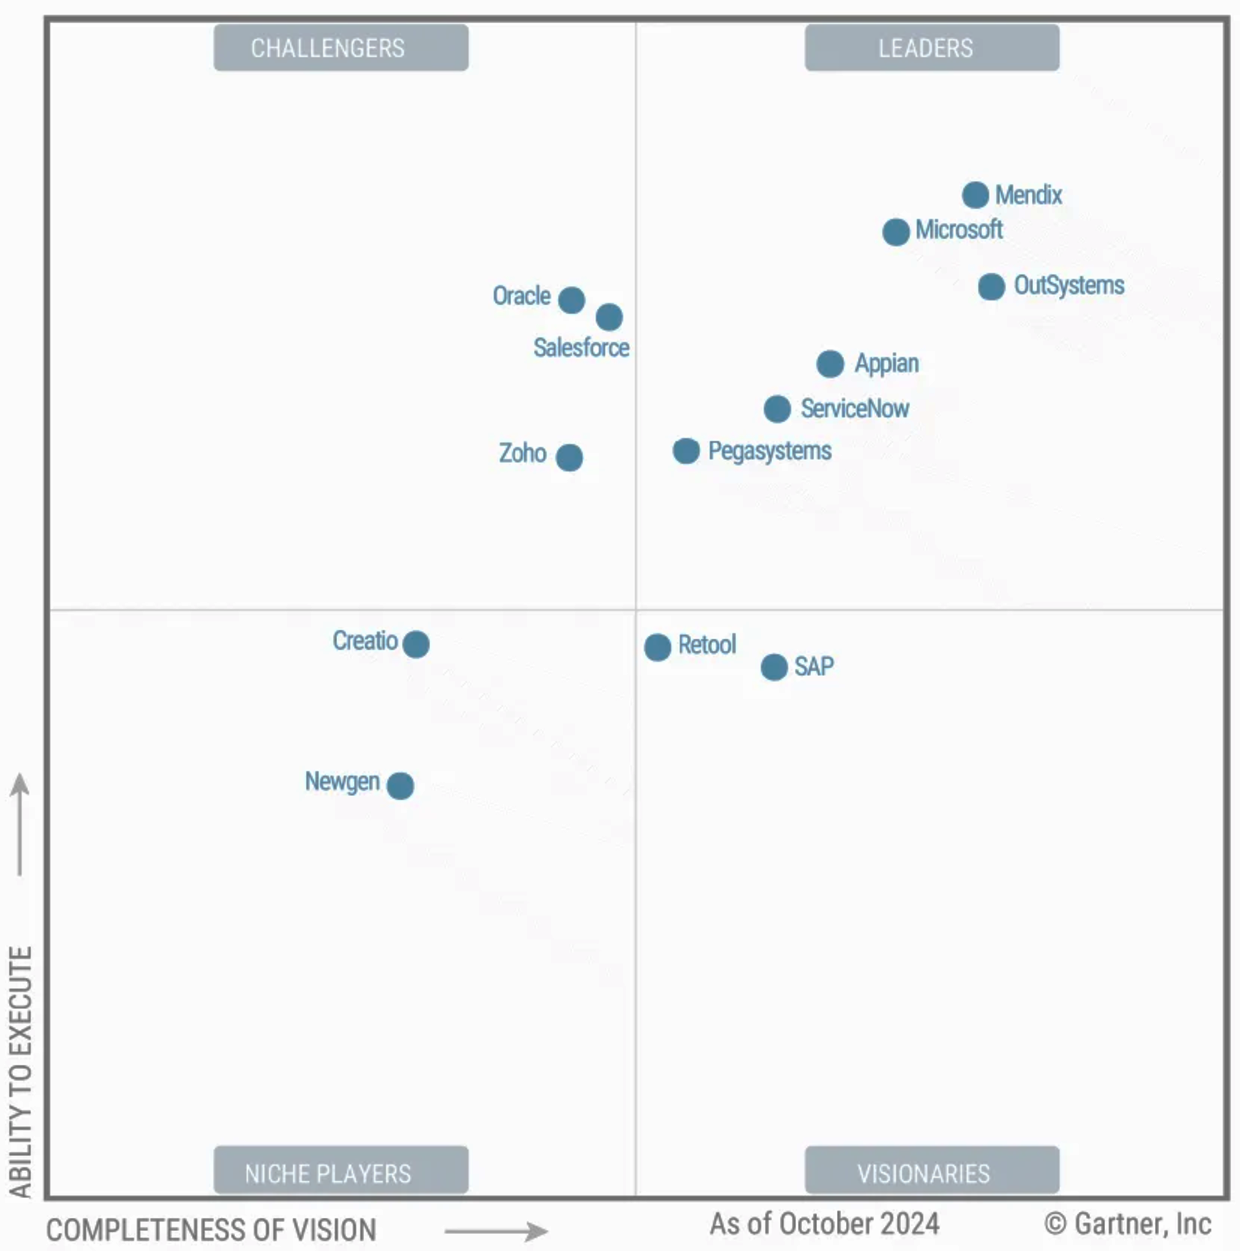
\includegraphics[width=0.5\textwidth]{GartnerQuadrant}
                    \caption{\centering Τεταρτημόριο της Gartner με πλατφόρμες ανάπτυξης λογισμικού \cite{mendixGartnerQuadrant}}
                    \label{fig:GartnerQuadrant}
            \end{figure}

    \section{Το Mendix Studio}
        Το Mendix Studio Pro επιτρέπει τη δημιουργία, προβολή και την ανάπτυξη εφαρμογών στην πλατφόρμα Mendix.

        \begin{figure}[h!] \noindent \centering
                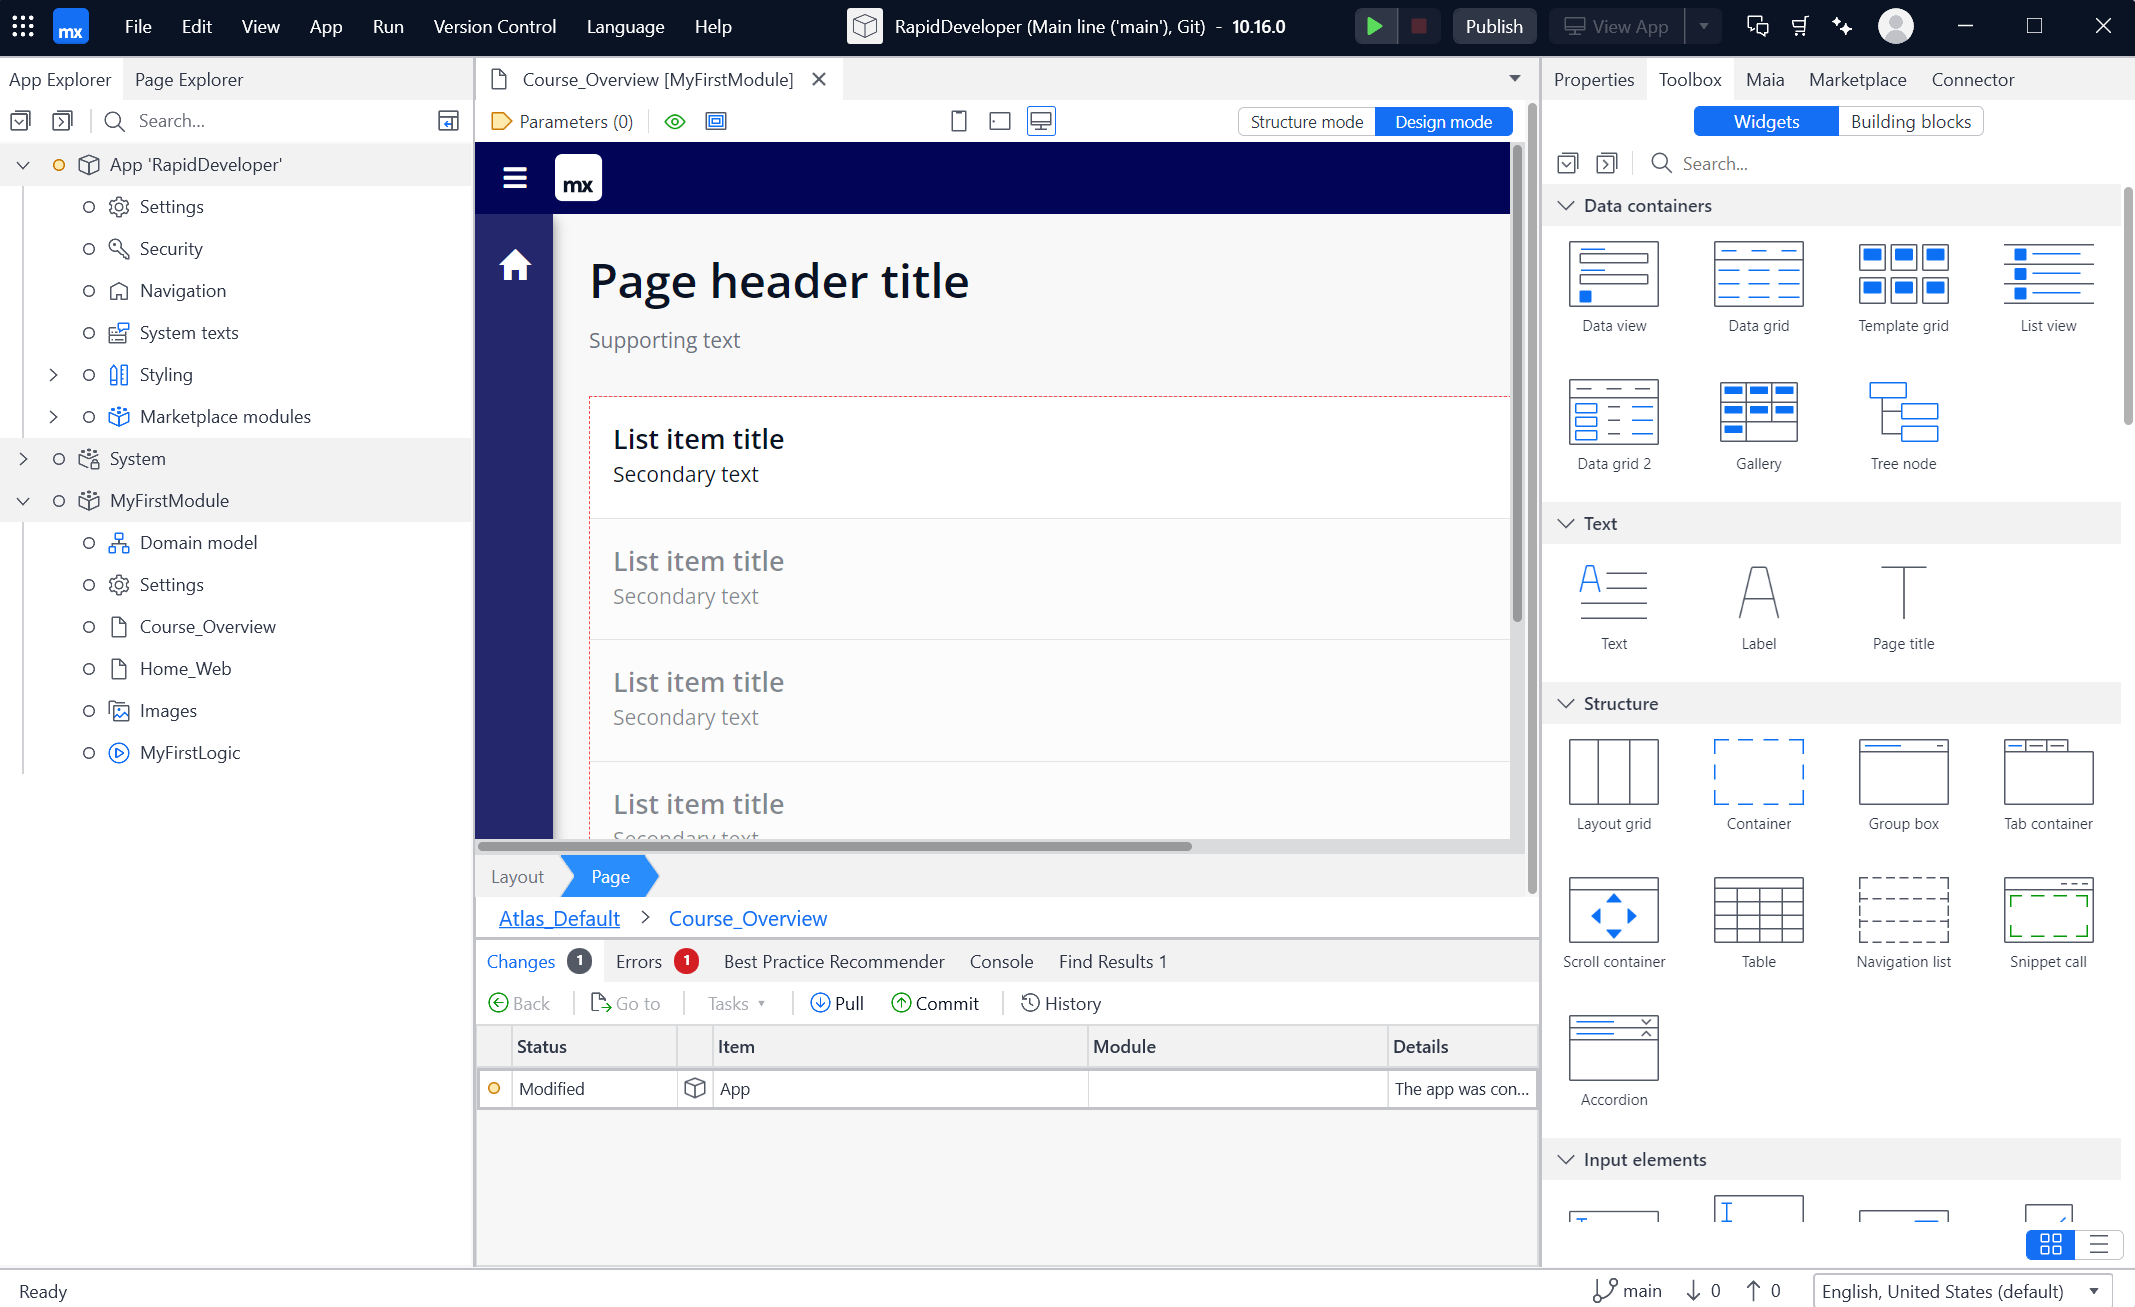
\includegraphics[width=\textwidth]{Mendix/MendixStudioOverlay}
                \caption{\centering Στιγμιότυπο του Mendix Studio Pro.}
                \label{fig:MendixStudioOverlay}
        \end{figure}

        \subsection{Περιβάλλον ανάπτυξης}
        Στο \ref{fig:MendixStudioOverlay} παρουσιάζεται το γραφικό περιβάλλον του Mendix Studio Pro με ανοιχτή την εφαρμογή \say{RapidDeveloper}\footnote{Η εφαρμογή RapidDeveloper δημιουργήθηκε ως αποτέλεσμα των μαθημάτων (crash courses) που προσφέρονται μέσω του Mendix Academy. Αυτά τα μαθήματα έχουν σχεδιαστεί για να παρέχουν στους χρήστες μια γρήγορη και πρακτική εισαγωγή στις βασικές δυνατότητες της πλατφόρμας Mendix, επιτρέποντάς τους να εξοικειωθούν με τη διαδικασία ανάπτυξης εφαρμογών σε περιβάλλον low-code.}.

        Μπορούμε να διαχωρίσουμε το γραφικό περιβάλλον σε τέσσερα μέρη. Η μαύρη μπάρα στο πάνω μέρος περιλαμβάνει το βασικό μενού του λογισμικού, το όνομα της εφαρμογής που αναπτύσσουμε, κουμπιά τα οποία επιτρέπουν είτε την τοπική εκτέλεση της εφαρμογής μέσω localhost ή τη διάθεσή της στο cloud, στο \textit{Mendix Sandbox}, και σύνδεσμοι που οδηγούν στο Mendix προφίλ του χρήστη, στο Marketplace κ.α.

        Στο κεντρικό τμήμα της οθόνης, κάτω από την επάνω μπάρα, βρίσκεται το \textit{Working Area}, όπου εμφανίζονται οι σελίδες της εφαρμογής μας. Στην αριστερή πλευρά, εντοπίζουμε τον \textit{App Explorer}, ο οποίος περιλαμβάνει τη δομή φακέλων και αρχείων της εφαρμογής, καθώς και τον \textit{Page Explorer}, που καταγράφει όλα τα στοιχεία που έχουν χρησιμοποιηθεί στη σελίδα της εφαρμογής που είναι ανοιχτή. Στη δεξιά πλευρά, βρίσκεται το \textit{Properties} Panel, όπου εμφανίζονται όλες οι ρυθμίσεις και οι παράμετροι των επιλεγμένων στοιχείων, και το \textit{Toolbox}, το οποίο περιέχει ένα σύνολο από προκατασκευασμένα στοιχεία που μπορούν να εισαχθούν στην εφαρμογή. Στο κάτω μέρος εμφανίζονται panels με τις αλλαγές που πραγματοποιούμε ανά commit, τα σφάλματα που υπάρχουν, logs, κονσόλα και άλλα. Μπορούμε σε οποιαδήποτε πεδίο να προσθέσουμε ή να αφαιρέσουμε Panels από το $ \text{Μενού} \rightarrow \text{View} $. \cite{mendixDoc}

        \subsubsection{Επιλογές για deployment} \label{sec:MendixDeployment}
            Το Mendix παρέχει διάφορες επιλογές για το deployment των εφαρμογών που αναπτύσσονται στην πλατφόρμα.

            Το Mendix Free δημιουργεί ένα δωρεάν online sandbox το οποίο επιτρέπει τη δημόσια διάθεση της αναπτυσσόμενης εφαρμογής. Το Mendix Free είναι κατάλληλο για την ανάπτυξη μικρών εφαρμογών και την εξοικείωση με την πλατφόρμα, αλλά δεν προσφέρει την απαιτούμενη ασφάλεια και ευελιξία για την ανάπτυξη μεγάλων επιχειρησιακύν εφαρμογών καθώς οι εφαρμογές παύουν να λειτουργούν μετά από λίγες ώρες αδράνειας (sleep mode), δεν μπορούν να κλιμακωθούν, υπάρχει όριο στην υπολογιστική ισχύ και το μέγεθος της βάσης δεδομένων, δεν τρέχουν προγραμματιζόμενα γεγονότα, δεν υποστηρίζονται custom domains κ.α. Παρόλα αυτά είναι μια πολύ καλή επιλογή που εξυπηρετεί τις ανάγκες των αρχάριων χρηστών και μικρών εφαρμογών. \cite{mendixCloud}

            Για χρήστες ή επιχειρήσεις με αυξανόμενες ανάγκες, το Mendix προσφέρει λύσεις επί πληρωμή που άρουν τους περιορισμούς που αναφέρθηκαν νωρίτερα.


    \section{Δομή εφαρμογών του Mendix}
        Μια εφαρμογή στο Mendix απαρτίζεται από διαφορετικά έγγραφα και modules. Τα modules ουσιαστικά διαχωρίζουν τη λειτουργικότητα της εφαρμογής σε αυτοτελή κομμάτια. Ο τρόπος με τον οποίο πραγματοποιείται ο διαχωρισμός εξαρτάται από την κρίση και τη σχεδιαστική προσέγγιση του μηχανικού λογισμικού.

        \subsection{Modules}
            Μια εφαρμογή περιλαμβάνει ένα \textit{System} module, modules που καθορίζονται από τους χρήστες ή modules από το Marketplace του Mendix, τα οποία μπορούν να προσφέρουν επιπλέον λειτουργικότητες κατασκευασμένες από τρίτους. Τέλος, μπορούμε να ορίσουμε modules με μοναδικό σκοπό τον καθορισμό της εμφάνισης της εφαρμογής (UI resources modules). Αυτά εμφανίζονται με πράσινο χρώμα και περιλαμβάνουν πρότυπα σελίδων (page templates) και δομικά στοιχεία (building blocks).

            Για παράδειγμα, στο App Explorer της εφαρμογής RapidDeveloper (σχήμα \ref{fig:MendixStudioOverlay}) παρατηρούμε πως εμφανίζονται τρία διαφορετικά modules: το module \say{App}, το module \say{System} και το module \say{MyFirstModule}. Τα δύο πρώτα είναι modules που δημιουργούνται αυτόματα κατά τη δημιουργία μιας εφαρμογής, ενώ το τρίτο είναι ένα module που δημιουργήθηκε από τον χρήστη.

            Κάθε module περιλαμβάνει ένα domain model που ορίζει τη δομή των δεδομένων του. Θα αναφερθούμε αναλυτικά στο domain model στην ενότητα \ref{sec:MendixDomainModel}.

            \subsubsection{Το module App}
            Στο module \say{App} μπορούν να επεξεργαστούν γενικές ρυθμίσεις που αφορούν την εφαρμογή. Συγκεκριμένα σε κάθε εφαρμογή του Mendix αντιστοιχούν πλαίσια διαλόγου για τις Ρυθμίσεις (Settings) της εφαρμογής, την Ασφάλεια (Security), την Πλοήγηση (Navigation), τα Κείμενα Συστήματος (System Texts)\footnote{Στο έγγραφο με τα Κείμενα Συστήματος μπορεί να γίνει μετάφραση των μηνυμάτων που παράγονται από τον διακομιστή κατά την εκτέλεση μιας εφαρμογής (για παράδειγμα \say{Password too short}).} και την Εξαγωγή Documentation (Export Documentation)\footnote{Στην Εξαγωγή Documentation μπορεί να εξαχθεί ένα HTML αρχείο με τα έγγραφα της εφαρμογής και το αντίστοιχο documentation.}.

            Οι Ρυθμίσεις περιλαμβάνουν παραμετροποιήσεις για το runtime της εφαρμογής, το theme που χρησιμοποιείται, την επιλογή συγκεκριμένων ενεργειών πριν αρχικοποιηθεί η εφαρμογή κατά την εκκίνησή της, επιλογή hash αλγορίθμων, γλώσσας και άλλα.

            \begin{figure}[h!] \noindent \centering
                    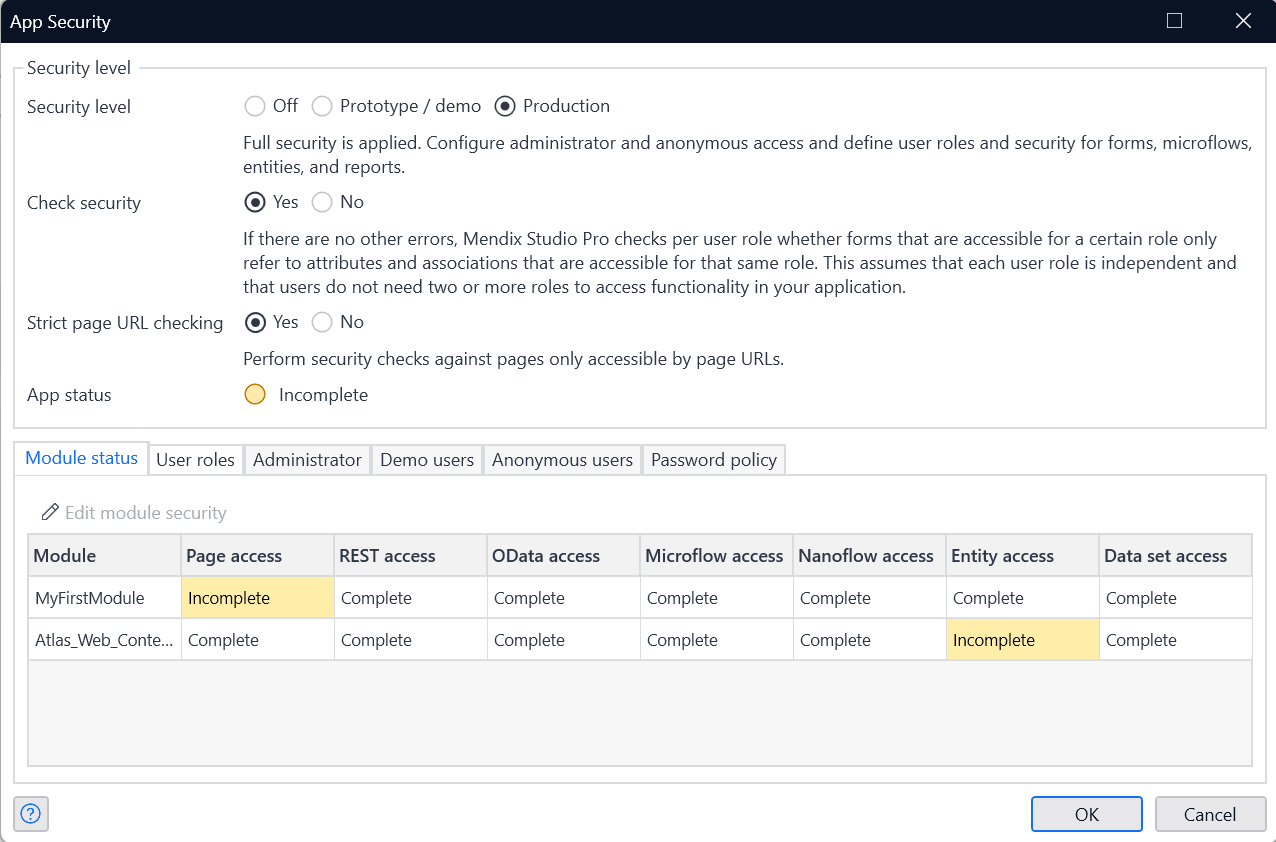
\includegraphics[width=0.8\textwidth]{Mendix/AppSecurity}
                    \caption{\centering Παράθυρο App Security.}
            \end{figure}

            Στην Ασφάλεια μπορούν να τροποποιηθεί το επίπεδο ασφάλειας (security level) της εφαρμογής (μπορεί να επιλεγεί ώστε οι χρήστες να μη χρειάζεται να συνδεθούν για να έχουν πρόσβαση ή να χρειάζεται σύνδεση), μπορούν να οριστούν ρόλοι χρηστών (δημιουργούνται ρόλοι στους χρήστες όπως Administrator, User, Guest και ανατίθενται τα modules και οι σελίδες στα οποία επιτρέπεται να έχουν πρόσβαση), διαπιστευτήρια του διαχειριστή της εφαρμογής (Adminstrator), ορίζονται demo χρήστες, ανώνυμοι χρήστες (οι οποίοι έχουν πρόσβαση στην εφαρμογή χωρίς να συνδεθούν) και να ρυθμιστούν κανόνες για τους κωδικούς πρόσβασης.

            \begin{figure}[h!] \noindent \centering
                    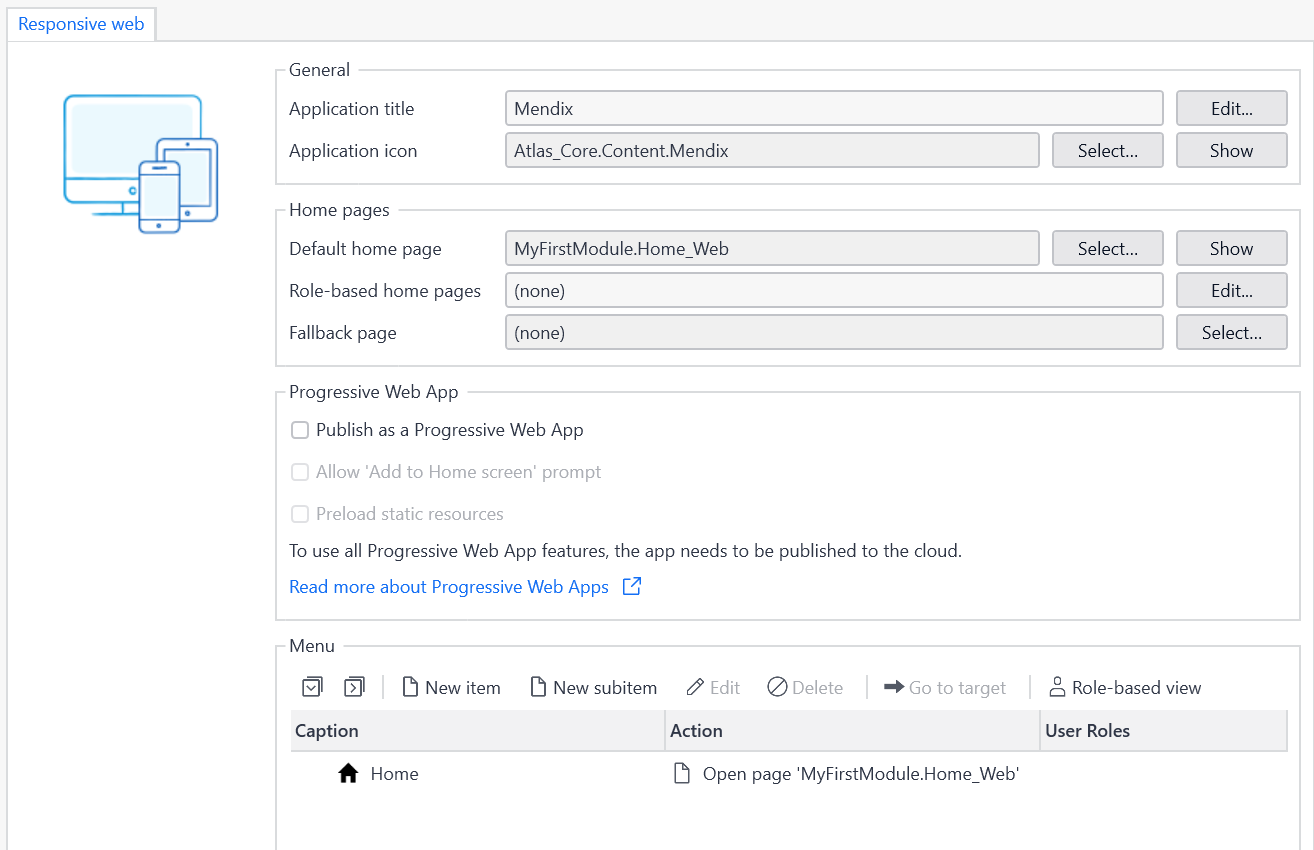
\includegraphics[width=0.8\textwidth]{Mendix/Navigation}
                    \caption{\centering To έγγραφο Navigation.}
            \end{figure}

            Στην Πλοήγηση μπορούν να διαμορφωθούν το όνομα και το εικονίδιο της εφαρμογής, η μπάρα μενού και η δομή του δέντρου πλοήγησης (navigation tree) και η αρχική σελίδα (home page) της εφαρμογής, η οποία μπορεί να είναι διαφορετική για κάθε ρόλο χρήστη. \cite{mendixDoc}

            \subsubsection{Το module System}
                Το module \say{System} είναι ένα προεγκατεστημένο module που περιλαμβάνει πολλές βασικές λειτουργίες της εφαρμογής. Παρέχει λειτουργικότητες όπως ζώνες ώρας, γλώσσες, ρόλους χρηστών, συνεδρίες (sessions) και άλλα. Το συγκεκριμένο module δεν μπορεί να επεξεργαστεί από τον χρήστη, αλλά μπορούν να προστεθούν συσχετίσεις (associations) ή γενικεύσεις (generalizations). Για παράδειγμα, μπορεί να δημιουργηθεί μια οντότητα \say{Πελάτης} η οποία θα συσχετίζεται με την οντότητα \say{Χρήστης} του module \say{System} και θα κληρονομεί τις ρυθμίσεις ασφαλείας του. \cite{mendixSystemModule}

        \subsection{Έγγραφα}
            Η Πλοήγηση είναι ένα \textit{έγγραφο} της εφαρμογής. Άλλα παραδείγματα εγγράφων είναι οι Σελίδες (Pages), τα Microflows και τα Enumerations\footnote{Τα enumerations καθορίζουν μια λίστα από προκαθορισμένες τιμές. Για παράδειγμα, ένα enumeration μπορεί να χρησιμοποιηθεί για τον καθορισμό της κατάστασης μιας εργασίας: \say{To do}, \say{Done} ή \say{Doing}.}.

        \subsection{Σελίδες}
            Η δημιουργία μιας σελίδας μπορεί να βασιστεί σε πόρους που προέρχονται από έγγραφα, όπως οι Εικόνες (Images), τα Layouts που καθορίζουν τη διάταξη της σελίδας, τα Μενού (Menus) που διαμορφώνουν την πλοήγηση, ή τα Snippets, τα οποία αποτελούν επαναχρησιμοποιήσιμα τμήματα διεπαφής.\footnote{Το Mendix είναι μια Εφαρμογή Μίας Σελίδας (Single-page application -- SPA) που σημαίνει ότι όλη η αλληλεπίδραση πραγματοποιείται σε μία μόνο καρτέλα ή παράθυρο του προγράμματος περιήγησης που φορτώνεται μία φορά και στη συνέχεια ενημερώνεται δυναμικά χωρίς να χρειάζεται να φορτωθεί ξανά. Ως αποτέλεσμα, δεν είναι δυνατή η ανοίγματος νέων σελίδων σε διαφορετική καρτέλα ή παράθυρο.}

            \subsubsection{Layout}
            Κάθε σελίδα στο Mendix βασίζεται σε ένα προκαθορισμένο layout, το οποίο καθορίζει βασικές ιδιότητες της σελίδας, όπως το μήκος, το πλάτος ή για παράδειγμα αν πρόκειται για αναδυόμενη (popup) σελίδα. Επιπλέον, τα layouts επιτρέπουν τον ορισμό στατικών τμημάτων, όπως ένα header ή ένα μενού, που παραμένουν σταθερά σε όλες τις σελίδες που τα χρησιμοποιούν. Το Mendix παρέχει επίσης έτοιμα πρότυπα σελίδων (Page Templates), τα οποία διευκολύνουν τη γρήγορη και απλή δημιουργία σελίδων με προκαθορισμένη δομή και σχεδίαση.

            \subsubsection{Widgets}
                Κάθε πρότυπο (Template), καθώς και κάθε σελίδα, αποτελείται από διάφορα στοιχεία (widgets). Ενδεικτικά παραδείγματα widgets περιλαμβάνουν:

                \begin{itemize}[label={\tiny \blacksquare}]
                    \setlength\itemsep{-0.25em}
                    \item Data containers -- δομές δεδομένων που περιέχουν δεδομένα από τη βάση δεδομένων. Παραδείγματα είναι Data view, Data grid, List view κ.α.
                    \item Text widgets -- περιέχουν κείμενο. Παραδείγματα είναι Text, Label, Page Title κ.α.
                    \item Structure widgets -- δομικά στοιχεία που χρησιμοποιούνται για την οργάνωση των widgets στη σελίδα. Παραδείγματα είναι Layout grid, Container, Tab container, Snippet call, Table κ.α.
                    \item Input widgets -- πεδία εισόδου δεδομένων. Παραδείγματα είναι Text box, Text area, Check box, Radio button, Drop-down, Date picker, File uploader κ.α.
                    \item Images, Videos ή Files -- widgets που περιέχουν πολυμέσα.
                    \item Buttons -- widgets που εκτελούν ενέργειες. Το Mendix παρέχει αρκετά buttons με προκαθορισμένες ενέργειες για την εκτέλεση ενεργειών όπως Save, Cancel, Delete, New, Edit, Crate, Call microflow κ.α.
                \end{itemize}

            \begin{figure}[h!] \noindent \centering
                    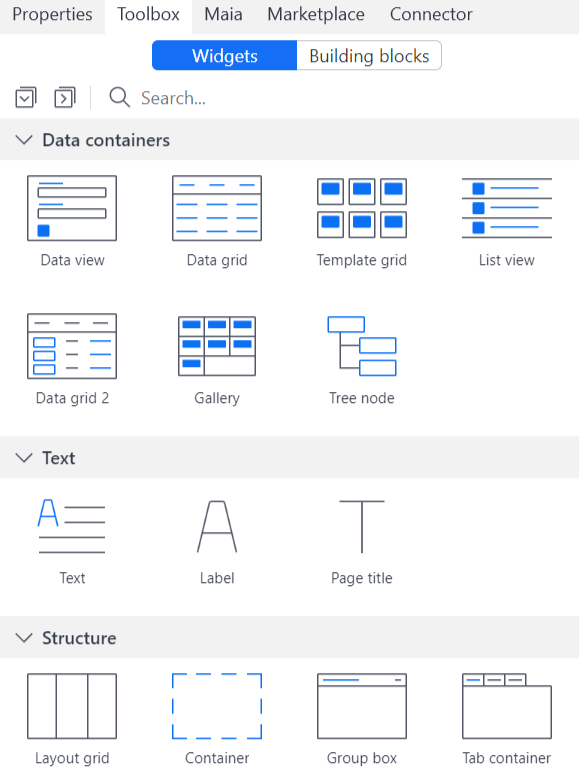
\includegraphics[width=0.3\textwidth]{Mendix/ToolboxPage}
                    \caption{\centering Τα Widgets περιλαμβάνονται στο Toolbox panel.}
            \end{figure}

                Τέλος, το Mendix προσφέρει προκαθορισμένα σύνολα Widgets, γνωστά ως Building Blocks, τα οποία περιλαμβάνουν στοιχεία όπως επικεφαλίδες (headers), φόρμες και ειδοποιήσεις (notifications). Αυτά τα Building Blocks διευκολύνουν και επιταχύνουν τη διαδικασία ανάπτυξης, παρέχοντας στους χρήστες έτοιμες λύσεις που μπορούν να ενσωματωθούν απευθείας στις εφαρμογές.

        \subsubsection{Εμφάνιση σελίδων}
            Στο Mendix Studio Pro, μια σελίδα μπορεί να προβληθεί είτε σε Structure Mode είτε σε Design Mode. Στο Structure Mode, παρουσιάζονται με σαφήνεια όλα τα δομικά στοιχεία που συνθέτουν τη σελίδα, ενώ στο Design Mode η σελίδα απεικονίζεται όπως θα εμφανίζεται στον τελικό χρήστη. Επιπλέον, το Design Mode περιλαμβάνει το X-Ray Mode, το οποίο συνδυάζει στοιχεία και από τις δύο άλλες λειτουργίες.

            \begin{figure}[h!] \noindent \centering
                    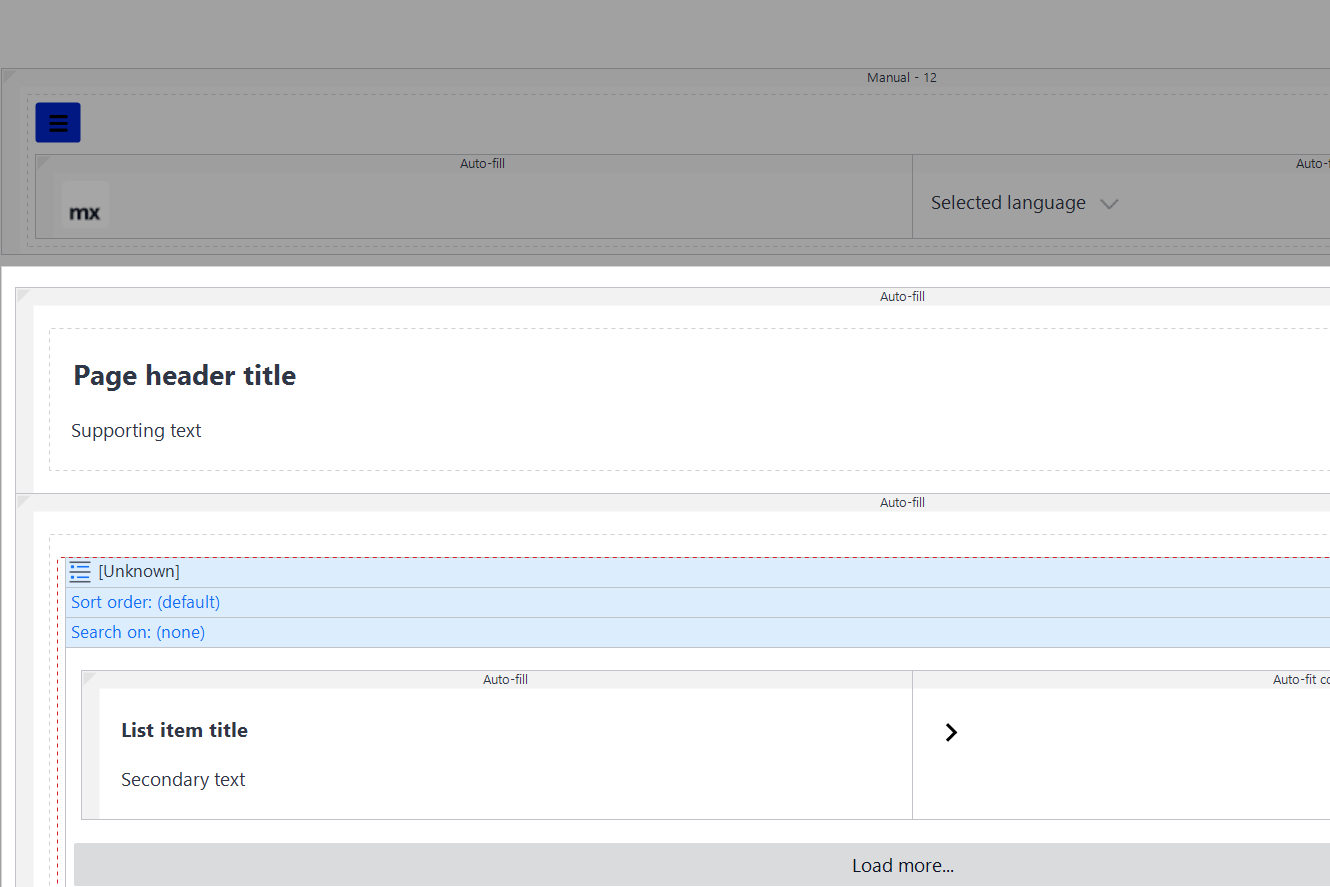
\includegraphics[width=0.32\textwidth]{Mendix/PageView2}
                    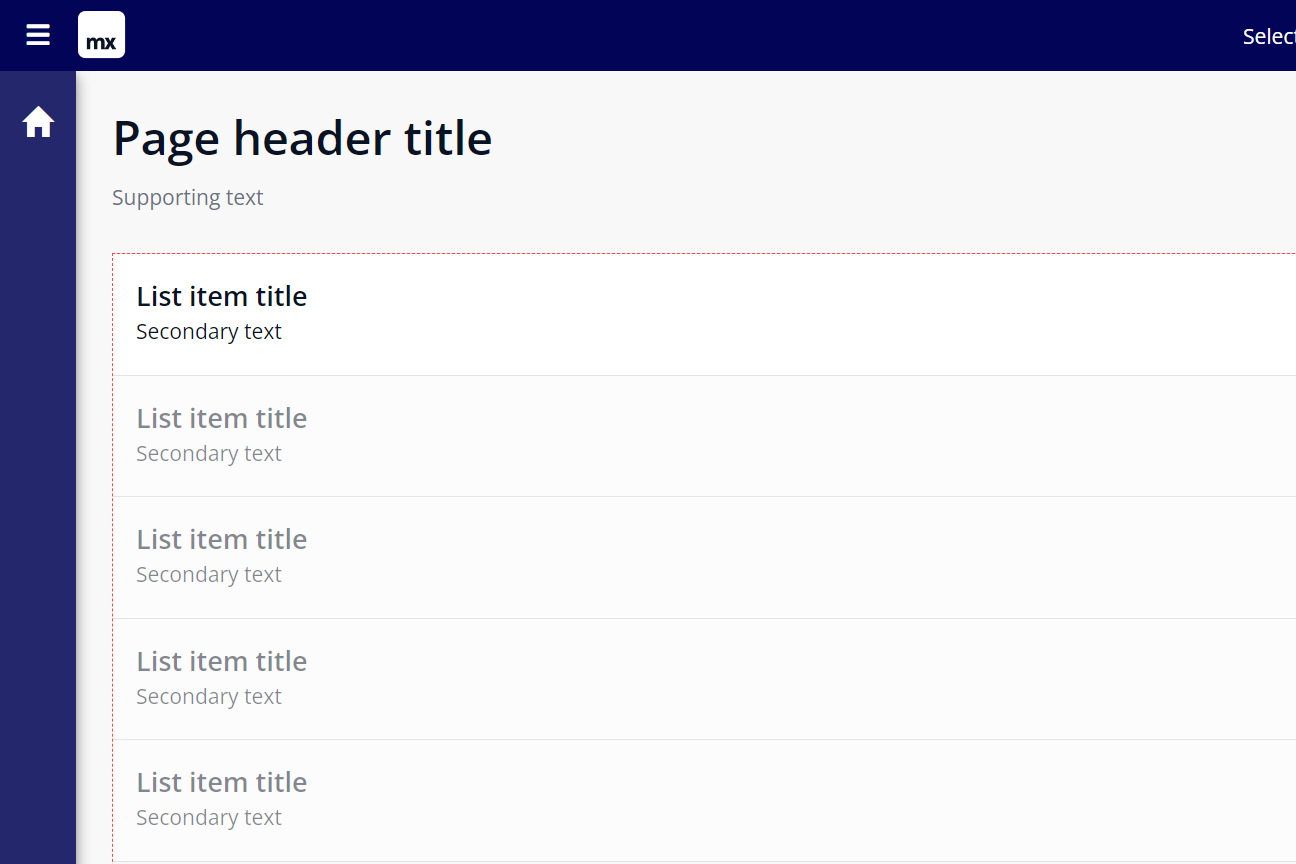
\includegraphics[width=0.32\textwidth]{Mendix/PageView1}
                    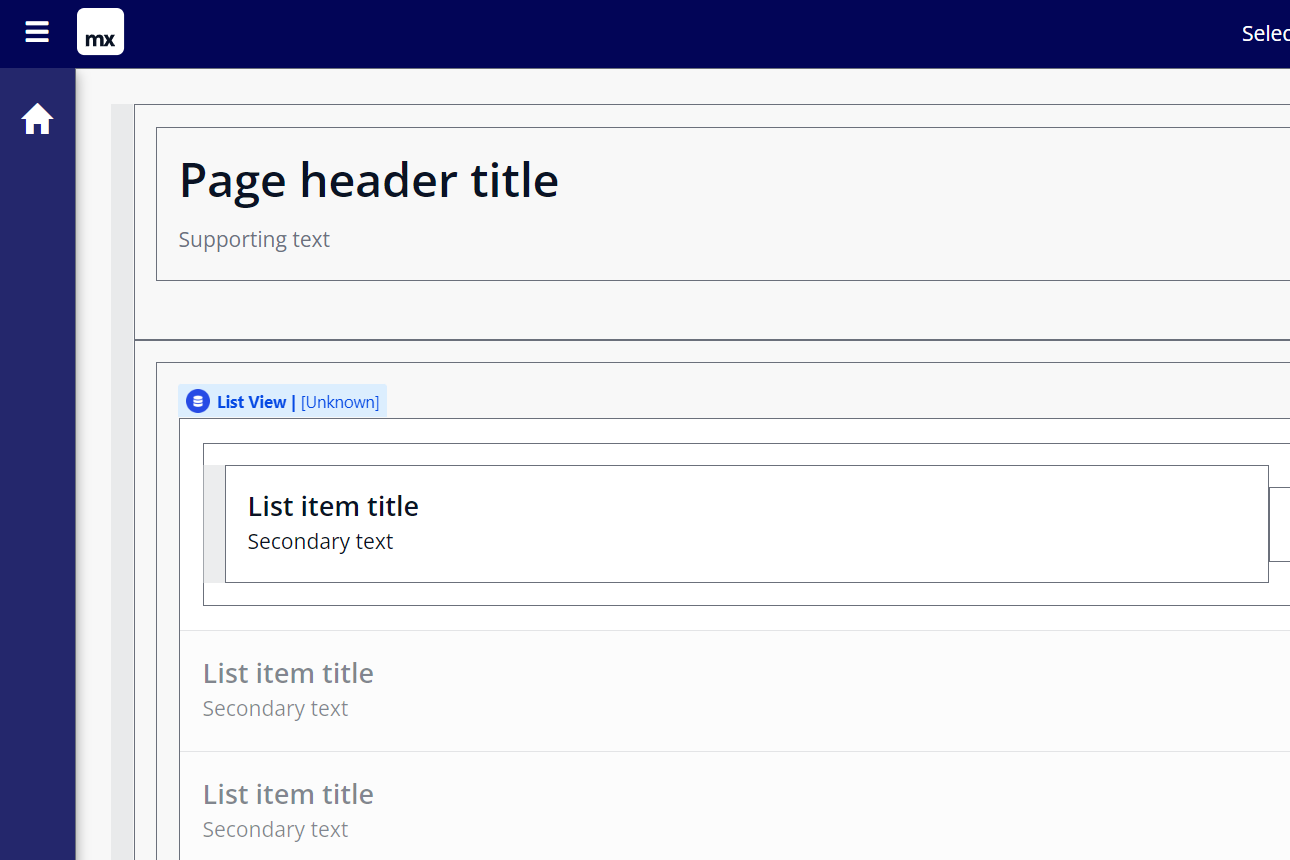
\includegraphics[width=0.32\textwidth]{Mendix/PageView3}
                    \caption{\centering Διαφορετικές εμφανίσεις της ίδιας σελίδας από αριστερά \\ προς τα δεξιά: Structure Mode, Design Mode, X-Ray Mode.}
            \end{figure}

        \subsection{Microflows}
            Τα Microflows (όπως και τα Nanoflows και τα Workflows)\footnote{Η βασική διαφορά μεταξύ Microflows και Nanoflows έγκειται στη λειτουργικότητα και τον τρόπο εκτέλεσής τους. Τα Microflows βασίζονται σε βιβλιοθήκες της Java, εκτελούνται στον διακομιστή (runtime server) και, ως εκ τούτου, δεν είναι διαθέσιμα για εφαρμογές που λειτουργούν εκτός σύνδεσης. Από την άλλη πλευρά, τα Nanoflows χρησιμοποιούν βιβλιοθήκες της JavaScript, εκτελούνται στην πλευρά του client, γεγονός που τα καθιστά εν δυνάμει γρηγορότερα.

Τα Microflows είναι ιδανικά για την προσκόμιση και την επεξεργασία δεδομένων από τη βάση δεδομένων ή από εξωτερικές πηγές, εξασφαλίζοντας υψηλή αξιοπιστία και συνέπεια. Αντίθετα, τα Nanoflows χρησιμοποιούνται κυρίως για ενέργειες που σχετίζονται με την εμπειρία του χρήστη, όπως η εμφάνιση αναδυόμενων (pop-up) μηνυμάτων, η προβολή progress bars ή η ανταλλαγή cookies.

Τέλος, τα Workflows ενδείκνυνται για τη διαχείριση σταθερών και επαναλαμβανόμενων διαδικασιών, επιτρέποντας την αυτοματοποίηση και την απλοποίηση της εκτέλεσής τους.} χρησιμοποιούνται για να εκφράσουν τη λογική της εφαρμογής. Είναι το κομμάτι του χαμηλού κώδικα που αναφέραμε στο κεφάλαιο \ref{ch:low-code} καθώς είναι ένας οπτικός τρόπος για την αναπαράσταση της λογικής της εφαρμογής. Ένα Microflow χρησιμοποιείται για να πραγματοποιήσει ενέργειες όπως η δημιουργία και η ενημέρωση αντικειμένων, η εμφάνιση σελίδων, το φιλτράρισμα δεδομένων, έλεγχος λειτουργικότητας κ.α.

            Κάθε Microflow αποτελείται από τα παρακάτω στοιχεία:
                \begin{itemize}[label={\tiny \blacksquare}]
                    \setlength\itemsep{-0.25em}
                    \item Events -- τα σημεία εκκίνησης και λήξης του Microflow.
                    \item Decisions -- συνθήκες που καθορίζουν τη ροή του Microflow.
                    \item Activities -- οι ενέργειες που πραγματοποιούνται στο Microflow. Για παράδειγμα, δημιουργία αντικειμένων (Create object), ενημέρωση αντικειμένων (Change object), διαγραφή αντικειμένων (Delete object), εμφάνιση σελίδων (Show page) κ.α.
                    \item Loops -- επαναλαμβανόμενες ενέργειες.
                    \item Parameter - δεδομένα εισόδου του Microflow.
                \end{itemize}

            \begin{figure}[h!] \noindent \centering
                    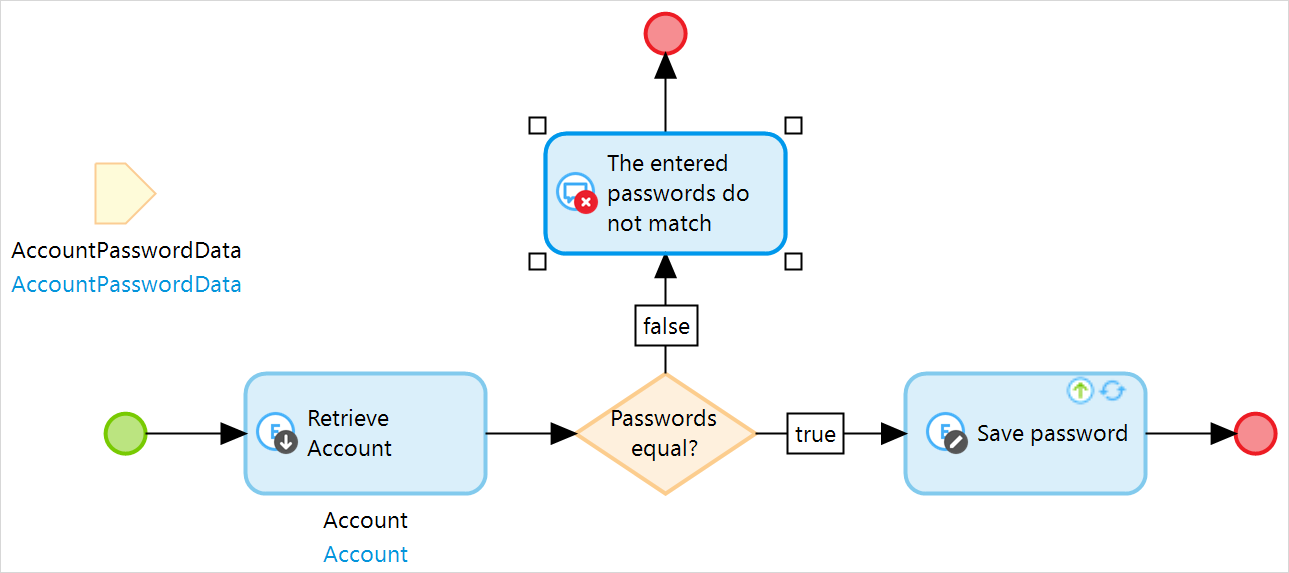
\includegraphics[width=0.7\textwidth]{Mendix/microflow-nanoflow-example}
                    \caption{\centering Παράδειγμα Microflow. Τα πράσινα και κόκκινα κυκλάκια αναπαριστούν τα events, τα μπλε ορθογώνια τα activities και ο πορτοκαλί ρόμβος το decision. Ως είσοδο έχουμε το parameter AccountPasswordData \cite{mendixDoc}.}
            \end{figure}

            Ένα Microflow μπορεί να εκτελεστεί από διαφορετικά μέρη όπως το Navigation menu, ένα κουμπί, ένα link ή ακόμα και από ένα άλλο Microflow. Επιπλέον, τα Microflows μπορούν να εκτελεστούν αυτόματα μετά από μια συγκεκριμένη ενέργεια (Event Handlers), όπως η αποθήκευση ενός αντικειμένου ή η ενημέρωση ενός πεδίου.

            \begin{figure}[h!] \noindent \centering
                    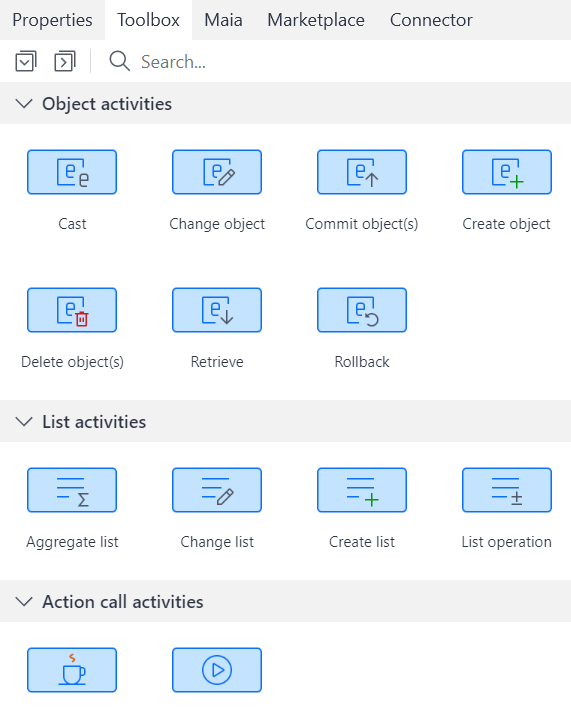
\includegraphics[width=0.3\textwidth]{Mendix/ToolboxMicroflow}
                    \caption{\centering Όταν επεξεργαζόμαστε ένα Microflow, to Toolbox panel περιλαμβάνει τα διαθέσιμα activities.}
            \end{figure}

        \subsection{Εκφράσεις}
            Οι εκφράσεις (expressions) του Mendix είναι ένας τρόπος ενσωμάτωσης λειτουργικότητας στην εφαρμογή μας. Οι εκφράσεις μπορούν να περιλαμβάνουν σταθερές τιμές, μεταβλητές, συναρτήσεις, λογικές πράξεις, συγκρίσεις, επιλογές κ.α. Για παράδειγμα, μπορεί να οριστεί η εμφάνιση ενός συγκεκριμένου widget μόνο αν ισχύει μια συγκεκριμένη συνθήκη. Οι εκφράσεις μπορούν να χρησιμοποιηθούν σε πολλά σημεία της εφαρμογής, όπως στα Microflows, στις σελίδες, στα widgets, στα validations κ.α.

            Για παραδειγμα, η έκφραση \verb|if $package/weight < 1.00 then 0.00 else 5.00| ελέγχει το γνώρισμα \texttt{weight} της οντότητας \texttt{package} και επιστρέφει \texttt{0.00} αν το βάρος είναι μικρότερο από \texttt{1.00}, αλλιώς επιστρέφει \texttt{5.00}. Θα δούμε περισσότερες τέτοιες εκφράσεις στην πράξη στο κεφάλαιο \ref{ch:unitask}.


        \subsection{Domain Model} \label{sec:MendixDomainModel}

            Το domain model είναι ένα μοντέλο δεδομένων που αναπαριστά τη δομή των δεδομένων κάποιου module στην πλατφόρμα Mendix. Τα δεδομένα που περιγράφονται από το domain model αποθηκεύονται στη συνέχεια σε ένα σχεσιακό σύστημα βάσεων δεδομένων του Mendix.

            Το domain model αποτελεί κεντρικό πυλώνα της αρχιτεκτονικής κάθε εφαρμογής. Κάθε module έχει το δικό του domain model, και όλα τα modules μπορούν να χρησιμοποιούν δεδομένα από όλα υπόλοιπα domain modules μέσω συσχετίσεων.

            \begin{figure}[h!] \noindent \centering
                    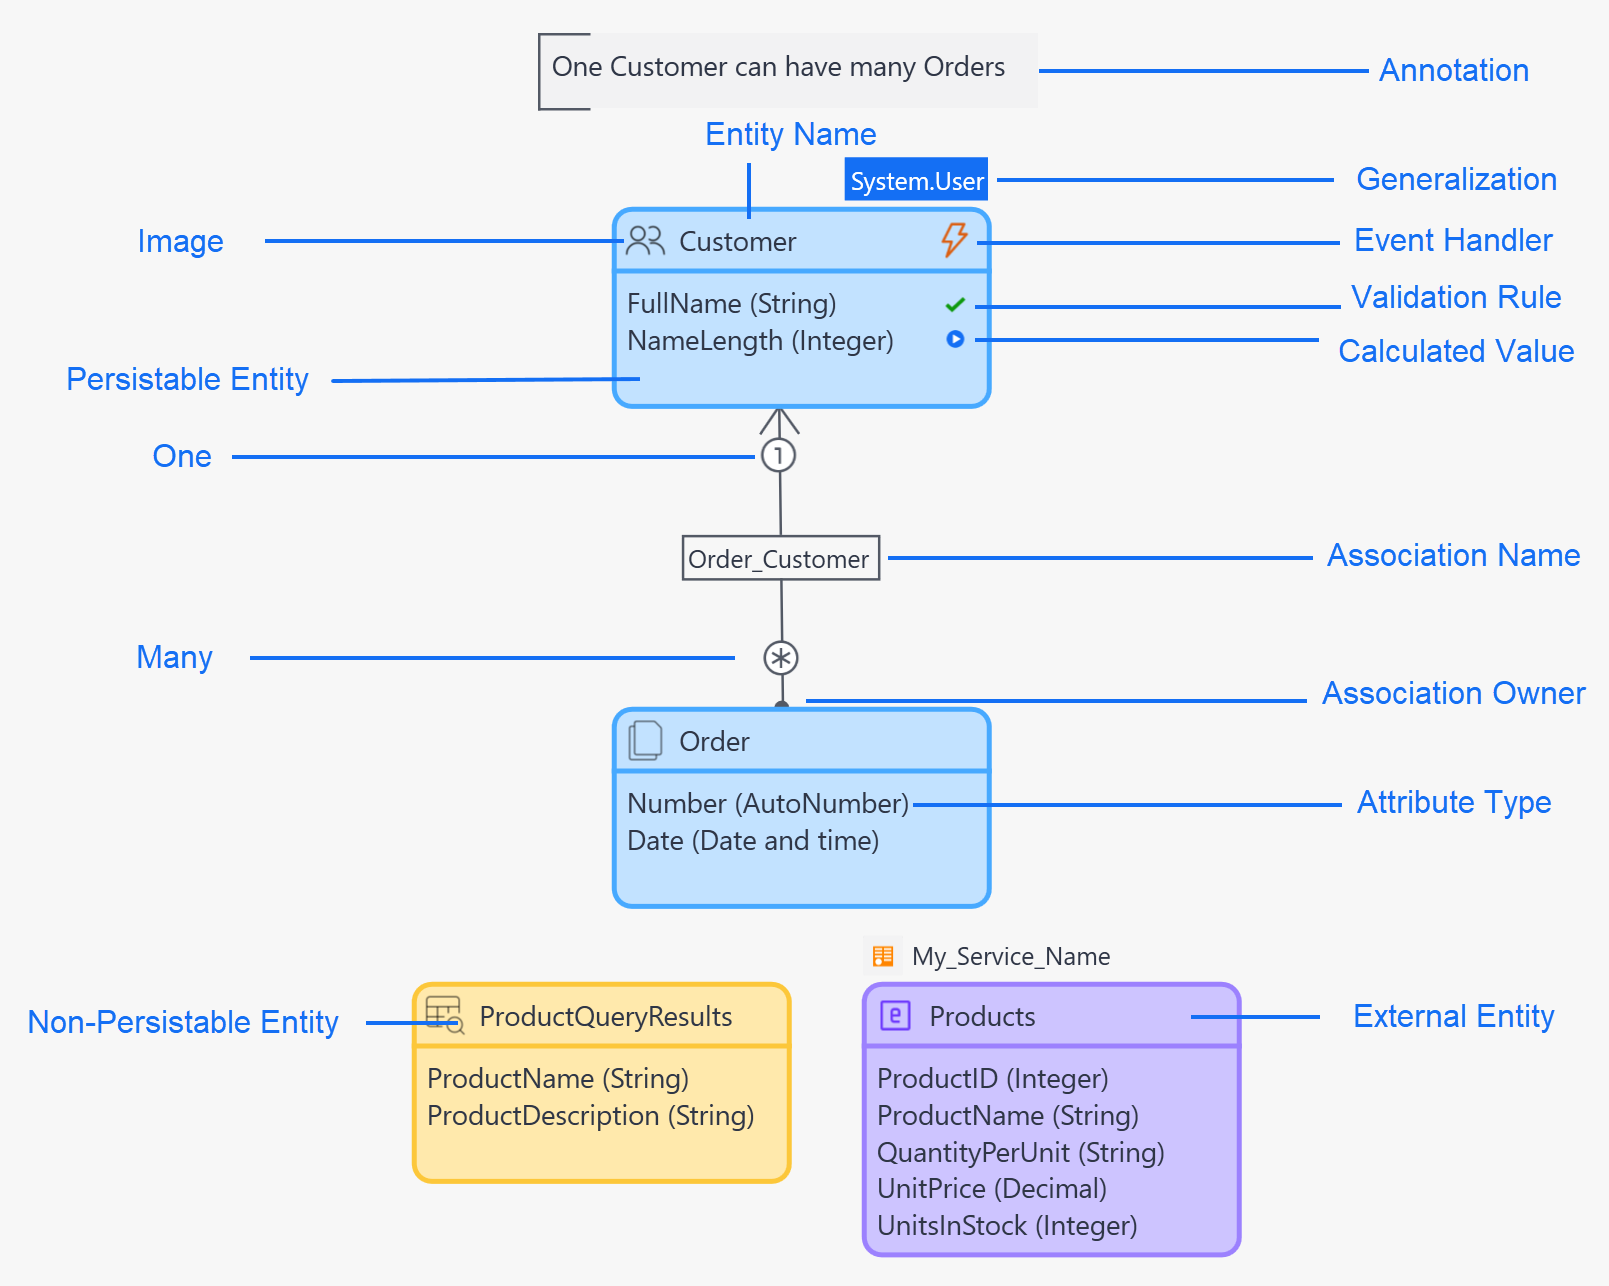
\includegraphics[width=0.8\textwidth]{Mendix/annotated-domain-model}
                    \caption{\centering Παράδειγμα από domain model. \cite{mendixDoc}}
                    \label{fig:MendixDomainModel}
            \end{figure}

            Το σχήμα \ref{fig:MendixDomainModel} είναι ένα παράδειγμα ενός domain model που αναπαριστά πελάτες και παραγγελίες. Οι πελάτες και οι παραγγελίες αποτελούν οντότητες (entities) του domain model. Οι οντότητες συσχετίζονται μεταξύ τους με μια συσχέτιση (association) πολλών-προς-ένα. Κάθε παραγγελία ανήκει σε έναν μόνο πελάτη, ενώ ένας πελάτης μπορεί να έχει πολλές παραγγελίες. Φυσικά, το Mendix περιλαμβάνει και άλλες πληθικότητες, όπως συσχετίσεις ένα-προς-ένα όπως επίσης και πολλά-προς-πολλά. Επιπλέον, αν διαγραφτεί κάποια οντότητα μπορεί να ρυθμιστεί τι θα συμβεί με τις συσχετίσεις της (π.χ. να διαγραφούν και αυτές).

            Μέσα στα ορθογώνια που αναπαριστούν τις οντότητες βρίσκονται τα γνωρίσματα, οι ιδιότητες (attributes) των οντοτήτων. Στην παρένθεση κάθε γνωρίσματος καταγράφεται ο τύπος δεδομένων του. Παρατηρούμε πως υπάρχουν ορθογώνια με διαφορετικά χρώματα, κάτι που αντιστοιχεί σε διαφορετικού είδους οντότητες. Τα μπλε ορθογώνια αναπαριστούν οντότητες που αποθηκεύονται στη βάση δεδομένων, με κίτρινο μη-διατηρήσιμες οντότητες (non-persistent entities), δηλαδή οντότητες που δεν αποθηκεύονται στη βάση δεδομένων αλλά αποθηκεύονται προσωρινά στη μνήμη, και τέλος με μωβ οντότητες από εξωτερικές πηγές δεδομένων. Η μπλε ετικέτα \say{System.User} που συνοδεύει την οντότητα Customer δηλώνει πως η οντότητα αυτή βασίζεται σε μια άλλη οντότητα, την οντότητα User του module System (Γενίκευση -- Generalization)\footnote{Η έννοια της γενίκευσης στο Mendix βασίζεται σε μια λογική που θυμίζει την κληρονομικότητα (inheritance) στις αντικειμενοστραφείς γλώσσες προγραμματισμού, δηλαδή επιτρέπει σε μία οντότητα (entity) να κληρονομεί τις ιδιότητες και τις συσχετίσεις μιας άλλης υπεροντότητας, χρησιμοποιώντας τα χαρακτηριστικά και τις συσχετίσεις της, ενώ παράλληλα μπορεί να ορίσει πρόσθετες ιδιότητες ή συσχετίσεις που είναι μοναδικές για την ίδια. Η γενίκευση είναι ιδιαίτερα χρήσιμη καθώς συμβάλλει στη διατήρηση της ακεραιότητας και της ασφάλειας των δεδομένων. Για παράδειγμα, οι \say{Customers} που κληρονομούν τα γνωρίσματα της οντότητας \say{System.User}, ταυτόχρονα κληρονομούν και όλα τα χαρακτηριστικά ασφάλειας του User που το Mendix έχει προκατασκευάσει.}. Τέλος, ανάλογα αν στην οντότητα έχει οριστεί κάποιος Event handler ή αν σε κάποιο γνώρισμα υπάρχει κάποιο validation rule, το Mendix το αναγνωρίζει και το αναπαριστά με το αντίστοιχο σύμβολο.

            \subsubsection{Οντότητες}
                \begin{figure}[h!] \noindent \centering
                        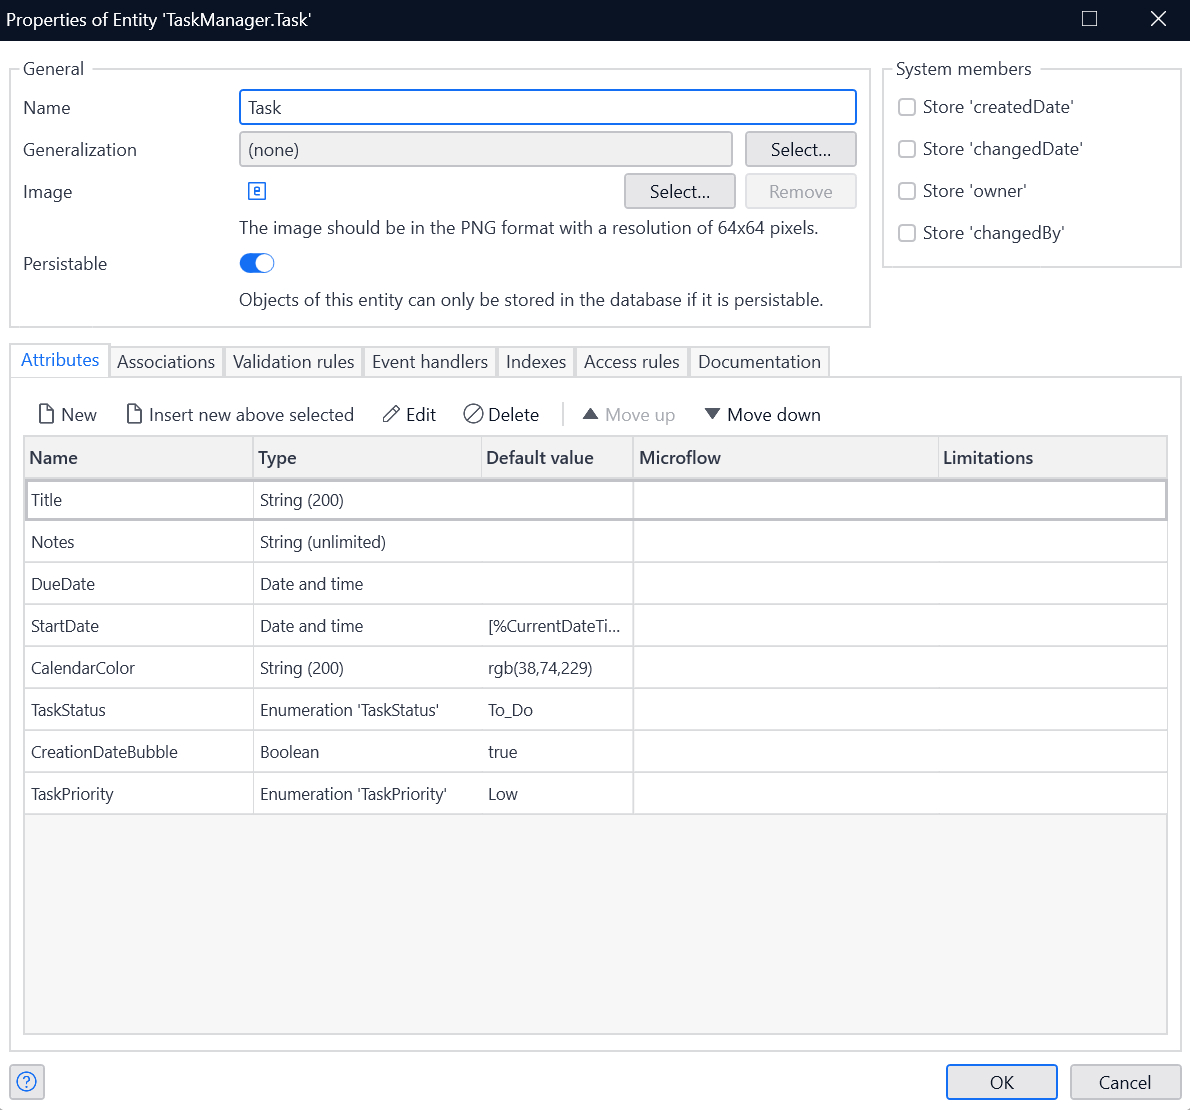
\includegraphics[width=0.8\textwidth]{Mendix/EntityProperties}
                        \caption{\centering Ιδιότητες μιας οντότητας Task (βλ. κεφ. \ref{ch:unitask})}
                        \label{fig:MendixEntityProperties}
                \end{figure}

                Στο σχήμα \ref{fig:MendixEntityProperties} παρουσιάζεται το παράθυρο που εμφανίζεται όταν δημιουργούμε ή επεξεργαζόμαστε μια οντότητα. Στο πάνω μέρος ορίζεται αν η οντότητα έχει κάποια γενίκευση και το αν είναι διατηρήσιμη στη βάση δεδομένων.

                Στην καρτέλα Attributes (Γνωρίσματα) καθορίζονται όλα τα γνωρίσματα της οντότητας. Εκεί επιλέγεται ο τύπος δεδομένων του γνωρίσματος. Οι τύποι δεδομένων που υποστηρίζονται από το Mendix είναι οι εξής: AutoNumber (αυτόματα παραγόμενοι αριθμοί, π.χ. IDs), Binary, Boolean, Date and time, Decimal, Enumeration (επιλέγεται κάποιο Enumeration έγγραφο), Hashed string, Integer, Long, String. Ο τύπος ενός γνωρίσματος είναι πιθανό να καθοριστεί αυτόματα από το Mendix βάσει του όνοματος που επιλέγεται κατά τον ορισμό του. Τέλος, μπορεί να οριστεί μια προεπιλεγμένη τιμή του κάθε ορίσματος ή να οριστεί η τιμή να καθορίζεται από κάποιο microflow.

                \begin{figure}[h!] \noindent \centering
                        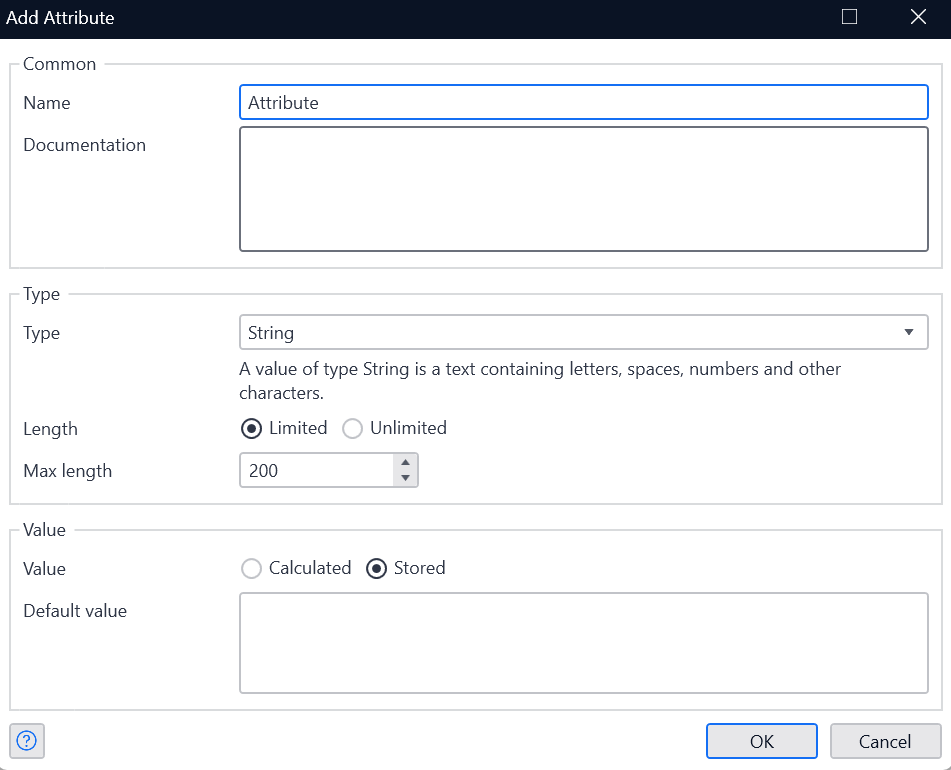
\includegraphics[width=0.6\textwidth]{Mendix/AddAttribute}
                        \caption{\centering Προσθήκη καινούριου γνωρίσματος σε μια οντότητα}
                \end{figure}

                Η καρτέλα Associations είναι ένας εναλλακτικός τρόπος που επιτρέπει να επεξεργαστούν οι συσχετίσεις μιας οντότητας. Ένας εναλλακτικός τρόπος είναι απευθείας από το domain model μέσω των συνδέσεων μεταξύ των οντοτήτων.

                Η καρτέλα Validation rules (Κανόνες Επικύρωσης) δημιουργεί συνθήκες που πρέπει να ικανοποιούνται για να είναι έγκυρα τα γνωρίσματα κάθε οντότητας. Οι κανόνες επικύρωσης μπορούν να είναι απλές συνθήκες, όπως π.χ. ένα πεδίο να μην είναι κενό, ή πιο σύνθετες, όπως π.χ. η τιμή ενός πεδίου να καθορίζεται από ένα εύρος τιμών.

                Η καρτέλα Event handlers (Χειριστές Συμβάντων) είναι ένας τρόπος για να εκτελεστούν συγκεκριμένες ενέργειες (microflows) όταν συμβεί κάποιο συγκεκριμένο συμβάν στην οντότητα. Τα συμβάντα μπορεί να είναι η δημιουργία (create), η ενημέρωση (commit ή save), η διαγραφή (delete) ή η ακύρωση (rollback ή cancel) μιας οντότητας. Μπορεί να επιλεγεί η εκτέλεση του microflow πριν ή μετά την εκτέλεση των παρακάτω συμβάντων.

                Η καρτέλα Access Rules (Κανόνες Πρόσβασης) ορίζει τα δικαιώματα χρήστης από κάθε ρόλο χρήστη όσον αφορά την αλληλεπίδραση με τα γνωρίσματα της οντότητας. Μπορεί να επιλεγεί ποιος ρόλος χρήστη μπορεί να δημιουργήσει ή να διαγράψει στιγμιότυπα από οντότητες και να διαβάσει ή να τροποποιήσει τα γνωρίσματά τους.

                \begin{figure}[h!] \noindent \centering
                        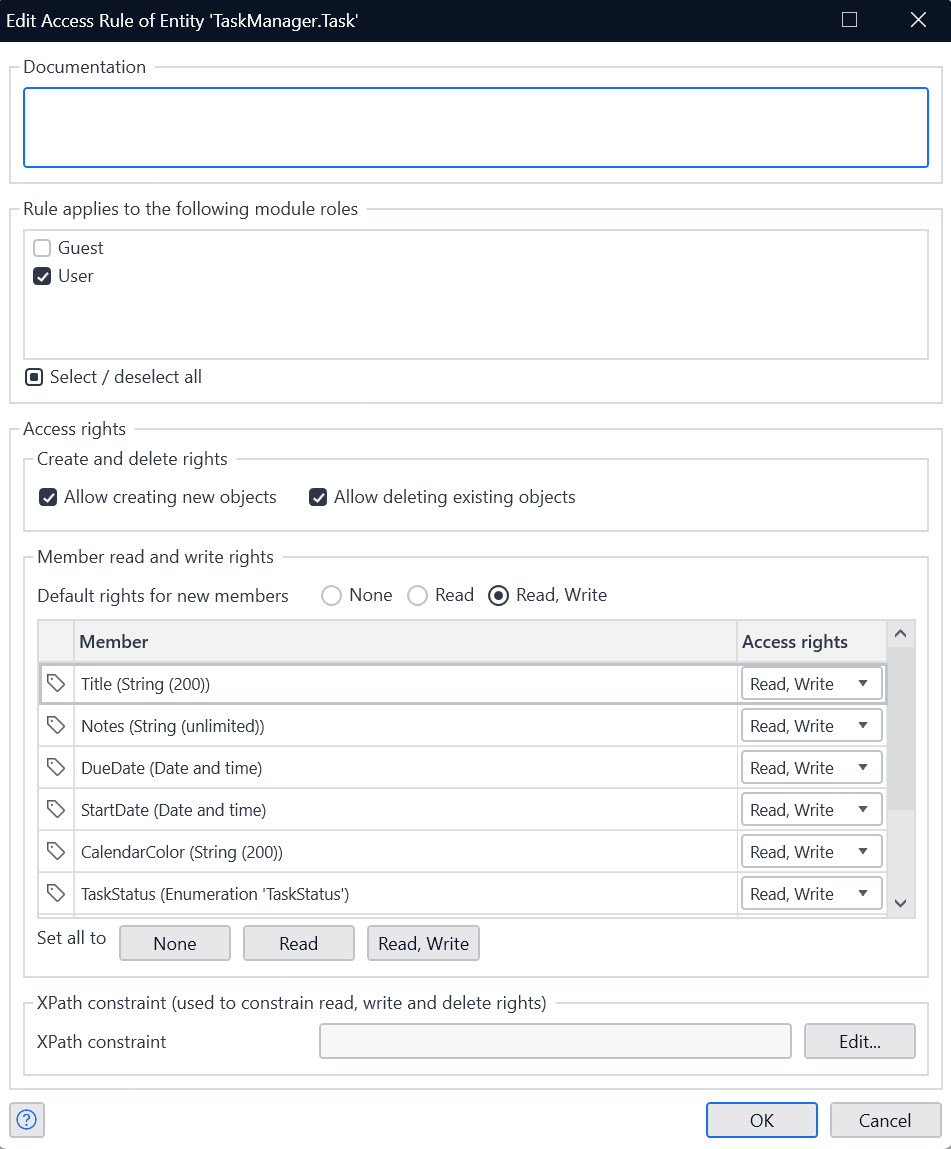
\includegraphics[width=0.6\textwidth]{Mendix/AccessRuleEntity}
                        \caption{\centering Επεξεργασία κανόνων πρόσβασης της οντότητας Task (βλ. κεφ. \ref{ch:unitask})}
                \end{figure}

                Τέλος οι καρτέλες Indexes και Documentation δημιουργούν δείκτες για την ταχύτερη ανάκτηση δεδομένων και παρέχουν documentation για την οντότητα αντίστοιχα.